\documentclass[../notes.tex]{subfiles}

\pagestyle{main}
\renewcommand{\chaptermark}[1]{\markboth{\chaptername\ \thechapter\ (#1)}{}}
\setcounter{chapter}{3}

\begin{document}




\chapter{Entropy and the Second Law of Thermodynamics}
\section{Entropy Equations}
\begin{itemize}
    \item \marginnote{1/31:}We define a new state function $S$ by $\dd{S}=\var{q_\text{rev}}/T$ and call it \textbf{entropy}.
    \begin{itemize}
        \item See notes from last time for why this is a state function.
    \end{itemize}
    \item Verify that the same definition of entropy is a state function for any system.
    \begin{itemize}
        \item Consider an ideal gas system in thermal equilibrium with an arbitrary system and drive the ideal gas system along a loop.
        \item Around the cycle: $\Delta S_\text{total}=0$.
        \item Ideal gas:
        \begin{align*}
            \Delta S_\text{total} &= \Delta S_1+\Delta S_2\\
            &= \int\frac{\var{q_{\text{rev}_1}}}{T}-\int\frac{\var{q_{\text{rev}_1}}}{T}\\
            &= \int\frac{\var{q_{\text{rev}_1}}}{T}+\int\frac{\var{q_{\text{rev}_2}}}{T}
        \end{align*}
    \end{itemize}
    \item We must devise a reversible process to calculate the entropy changes for an irreversible process leading to the same final state.
    \begin{figure}[h!]
        \centering
        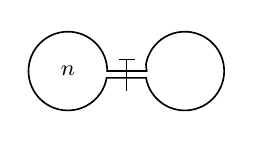
\begin{tikzpicture}
            \footnotesize
            \draw [semithick] (0.5,0) -- (0,0) arc[start angle=0,end angle=350,radius=5mm] -- ++(0.5,0) arc[start angle=-170,end angle=170,radius=5mm] -- cycle;
    
            \draw (0.25,-0.25) -- ++(0,0.4) ++(-0.1,0) -- ++(0.2,0);
    
            \node [left=3mm] {$n$};
        \end{tikzpicture}
        \caption{Two linked containers.}
        \label{fig:linkedContainers}
    \end{figure}
    \begin{itemize}
        \item Imagine two linked containers, one filled with $n$ moles of gas and the other vacuumed.
        \item Opening the two containers to each other results in an adiabatic expansion. All vibrational/rotational energy of the molecules is consumed and used for translation.
        \item Measuring the temperature with spectroscopy (the Maxwell-Boltzmann distribution of each spectral line, plus only the ground rovibrational states are occupied now) shows a drastic drop in temperature.
        \item We have $\var{q}=0$ and $\var{w}=0$ so that $\dd{U}=0$ and $\Delta T=0$ overall?
        \item An isothermal expansion is a reversible process leading to the same final state.
        \item $\dd{U}=0$ implies $\var{q_\text{rev}}=-\var{w}=P\dd{V}$.
        \item We have that
        \begin{equation*}
            \Delta S = \int\frac{\var{q_\text{rev}}}{T}
            = \int_{V_0}^{2V_0}\frac{P\dd{V}}{T}
            = \int_{V_0}^{2V_0}\frac{nRT}{V}\frac{1}{T}\dd{V}
            = nR\ln 2
        \end{equation*}
    \end{itemize}
    \item Using entropy as a state function to predict the vapor pressure in equilibrium with its liquid, from the enthalpy at boiling and the boiling temperature.
    \begin{figure}[h!]
        \centering
        \begin{tikzpicture}
            \footnotesize
            \node (a) at (0,0)  {\ce{H2O_{(l)}} $T  ,P_0$};
            \node (b) at (0,-2) {\ce{H2O_{(l)}} $T_b,P_0$};
            \node (c) at (4,-2) {\ce{H2O_{(g)}} $T_b,P_0$};
            \node (d) at (4,-1) {\ce{H2O_{(g)}} $T_b,P  $};
            \node (e) at (4,0)  {\ce{H2O_{(g)}} $T  ,P  $};
    
            \draw [-stealth,semithick] (a) -- node[above]{$\Delta S_0$} (e);
            \draw [-stealth,semithick] (a) -- node[left ]{$\Delta S_1$} (b);
            \draw [-stealth,semithick] (b) -- node[below]{$\Delta S_2$} (c);
            \draw [-stealth,semithick] (c) -- node[right]{$\Delta S_3$} (d);
            \draw [-stealth,semithick] (d) -- node[right]{$\Delta S_4$} (e);
        \end{tikzpicture}
        \caption{Vapor pressure thermodynamic loop.}
        \label{fig:thermodynamicLoop}
    \end{figure}
    \begin{itemize}
        \item Consider the above thermodynamic loop, where $T$ is the temperature of the water and $P$ is the pressure above the water.
        \item We have that
        \begin{align*}
            \Delta S_1 &= \int_T^{T_b}\frac{C_{P_l}}{T}\dd{T}&
            \Delta S_2 &= \frac{\Delta H_\text{vap}}{T_b}&
            \Delta S_3 &= nR\ln\frac{P_0}{P}&
            \Delta S_4 &= \int_{T_b}^T\frac{C_{P_g}}{T}\dd{T}
        \end{align*}
        and that
        \begin{equation*}
            \Delta S_0 = \frac{\Delta H_\text{vap}}{T}
        \end{equation*}
        \item We know that $\Delta S$ around the loop is zero since $S$ is a state function. We neglect the heat capacity effect. Thus,
        \begin{align*}
            \frac{\Delta H_\text{vap}}{T_b}+nR\ln\frac{P_0}{P}-\frac{\Delta H_\text{vap}}{T} &= 0\\
            \ln\frac{P_0}{P} &= \frac{\Delta H_\text{vap}}{nR}\left( \frac{1}{T}-\frac{1}{T_b} \right)\\
            P &= P_0\e[-\Delta H_\text{vap}/nR(1/T-1/T_b)]
        \end{align*}
        \item The above equation gives the vapor pressure at $T$ in terms of the vapor pressure $P_0$ at $T_b$.
    \end{itemize}
    \item \textbf{Trouton's rule}: The statement that
    \begin{equation*}
        \frac{\Delta H_\text{vap}}{T_b} \approx 85\pm\SI{5}{\joule\per\mole\per\kelvin}
    \end{equation*}
    \begin{itemize}
        \item Discovered this rule as an undergrad after an afternoon's manipulation of data from a book of tables.
        \item This rule reflects the fact that
        \begin{equation*}
            \frac{\Delta H_\text{vap}}{T_b} = \Delta S_\text{vap}
        \end{equation*}
        and implies that $\Delta S_\text{vap}$ is approximately a constant.
    \end{itemize}
    \item Example of entropy change: The direction of heat flow between two systems (1 and 2) only in thermal contact.
    \begin{itemize}
        \item We have
        \begin{align*}
            \var{q_{\text{rev}_1}} &= \var{q_{\text{rev}_2}}\\
            C_{V_1}\dd{T_1} &= -C_{V_2}\dd{T_2}
        \end{align*}
        \item Thus,
        \begin{align*}
            \dd{S} &= \dd{S_1}+\dd{S_2}\\
            &= \frac{\var{q_{\text{rev}_1}}}{T_1}+\frac{\var{q_{\text{rev}_2}}}{T_2}\\
            &= \frac{C_V\dd{T_1}}{T_1}-\frac{C_V\dd{T_1}}{T_2}\\
            &= C_V\dd{T_1}\left( \frac{1}{T_1}-\frac{1}{T_2} \right)
        \end{align*}
        \item The conclusion is that if $\dd{T_1}>0$, then $\dd{S}>0$. This is the spontaneous direction, the direction that nature chooses, the one in which entropy increases.
        \item The maximum of $S$ is the equilibrium temperature between the two systems.
    \end{itemize}
    \item Entropy change of the isothermal mixing of two ideal gases at the same temperature.
    \begin{itemize}
        \item Consider the same two-container setup from Figure \ref{fig:linkedContainers}.
        \item We have that
        \begin{align*}
            \Delta S &= Rn_1\ln\frac{V_1+V_2}{V_1}+Rn_2\ln\frac{V_1+V_2}{V_2}\\
            &= R(n_1+n_2)\left( \frac{n_1}{n_1+n_2}\ln\frac{V_1+V_2}{V_1}+\frac{n_2}{n_1+n_2}\ln\frac{V_1+V_2}{V_2} \right)\\
            &= R(n_1+n_2)(-y_1\ln y_1-y_2\ln y_2)\\
            &= R(n_1+n_2)[-y_1\ln y_1-(1-y_1)\ln(1-y_1)]
        \end{align*}
        \begin{itemize}
            \item Note that $y_1=n_1/(n_1+n_2)=V_1/(V_1+V_2)$ is the mole fraction, and similarly for $y_2$.
        \end{itemize}
        \item The conclusion is that $\Delta S>0$.
        \item The maximum of $\Delta S$ is at $y_1=y_2=1/2$.
    \end{itemize}
    \item \textbf{Gibb's paradox}: Suppose you have the same gas on both sides of the containers. Then $\Delta S=nR\ln 2$ for an indistinguishable gas.
    \begin{itemize}
        \item This is wrong.
        \item Resolved by knowing that the gases \emph{must} be distinguishable.
    \end{itemize}
\end{itemize}




\end{document}